\documentclass[a4paper]{article}

\usepackage{ReportTemplate}

\usepackage{setspace}
\usepackage{amsmath}
\usepackage[hidelinks]{hyperref}
\usepackage{algorithm}
\usepackage{algorithmicx}
\usepackage{algpseudocode}

\raggedbottom
\title{Project 1:语音端点检测}
\name{涂宇清}
\studentid{522030910152}

\begin{document}

\maketitle

% \section{LaTeX写作示例}

% 本章提供使用LaTeX书写报告时可能使用的各种文档对象的使用示例。\textbf{请在报告写作完成后删
% 除本章。}

% \subsection{公式}

% 示例如式\ref{eq:公式引用名}。

% \begin{equation}
%   \pi = \dfrac{3.1415926}{1}
%   \label{eq:公式引用名}
% \end{equation}

% \subsection{图像}

% 示例如图\ref{fig:图片引用名}。

% \begin{figure}[htb]
%   \centering
%   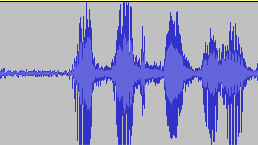
\includegraphics[scale=0.7]{figs/voice.png}
%   \caption{图片标题}
%   \label{fig:图片引用名}
% \end{figure}

% \subsection{表格}

% 示例如表\ref{tab:表引用名}。

% \begin{table}[th]
%   \caption{表标题}
%   \label{tab:表引用名}
%   \centering
%   \begin{tabular}{ l c r }
%     \toprule
%     \textbf{左对齐} & \textbf{居中对齐} & \textbf{右对齐} \\
%     \midrule
%     内容 & 内容 & 内容 \\
%     内容 & 内容 & 内容 \\
%     \bottomrule
%   \end{tabular}
% \end{table}

% \subsection{代码}

% 示例如下。

% \begin{lstlisting}[language=python]
% # 这是注释
% def func(a, b):
%     print("Hello, world!")
% \end{lstlisting}

\section{基于线性分类器和语音短时能量的简单语音端点检测算法}

\subsection{数据预处理及特征提取}

% 本节介绍任务1中你对输入数据进行了哪些预处理步骤,提取了什么特征。对每种预处理步骤,请简要
% 介绍该步骤的效果或功能;对每种特征,请简要介绍该特征的定义和/或该特征对人耳听觉造成的直观
% 感受。\textbf{写作完成后,请删除本段。}

\subsubsection{数据预处理}

使用\verb|wavfile.read()|读取音频文件后,将其按照帧长32ms和帧移8ms进行分帧。对于文件末尾长度不足的帧,使用\verb|np.append()|函数补零。

分帧后,使用汉明窗对每一帧进行加窗处理,强调了每一帧信号的局部中心特性,抑制了一些无关边际特性对全局特征的影响。

\subsubsection{短时能量}

短时能量是语音信号的一种重要特征,为一帧内采样点幅值的平方和,可反映短时间内音频的能量大小。短时能量的计算公式如下:
\[E=\sum_{i=0}^{N-1}s_n^2\]
其中$E$为一帧的短时能量,$N$为一帧的采样点数,$s_n$为第$n$个采样点的幅值。

\subsubsection{过零率}
过零率是语音信号的另一种重要特征,为每一帧采样点正负反复的次数,可反映语音信号的频率大小。过零率的计算公式如下:
\[Z=\frac{1}{2}\left\{\sum_{n=0}^{N-1}|sgn\left[s\left(n\right)\right]-sgn\left[s\left(n-1\right)\right]|\right\}\]
其中$Z$为一帧的过零率,$N$为一帧的采样点数,$s(n)$为第$n$个采样点的幅值,$sgn()$为符号函数。

\subsection{算法描述}

% 请描述你的语音端点检测算法。若不止一种,可继续分节。请尽可能使用伪代码描述。如有必要,可以
% 贴出少量程序代码。\textbf{写作完成后,请删除本段。}

\subsubsection{阈值分类器}

阈值分类器是一种简单的分类器,通过设置一个阈值,当短时能量和过零率超过阈值时,判断为语音信号,否则判断为非语音信号。

\begin{algorithm}[H]
    \caption{阈值分类器}
    \begin{algorithmic}[1]
        \State\textbf{输入:}一帧的短时能量、过零率,短时能量阈值$thres_0$、过零率阈值$thres_1$
        \State\textbf{输出:}这一帧是否为语音信号
        \If{短时能量$>thres_0$\ $\wedge $过零率$>thres_1$}
        \State\Return{$1$}
        \Else
        \State\Return{$0$}
        \EndIf
    \end{algorithmic}
\end{algorithm}

由参数调节得,短时能量阈值为35000,过零率阈值为0.005时,对语音信号的检测效果较好。

\subsubsection{优化预测结果}

在对每帧语音进行阈值分类时,我们并没有考虑到语音信号的连续性。因此,我们可以对预测结果进行优化,从而减少预测结果中的断点,并补全短时能量与过零率难以判断的语音清音区。

\begin{algorithm}[H]
    \caption{优化预测结果}
    \begin{algorithmic}[1]
        \State\textbf{输入:}预测结果,平滑阈值$sl$, 清音区长度$n$
        \State\textbf{输出:}优化后的预测结果
        \If{一组连续标签为0的帧的数量$<$\ $sl$}
        \State{这组连续标签为0的帧全部标记为1}
        \EndIf
        \For{每一段全部被标记为1的连续语音段}
        \State{分别将这个语音段前后的$n$个标记为0的帧标记为1}
        \EndFor
    \end{algorithmic}
\end{algorithm}

由参数调节得,平滑阈值为17,清音区长度为3时,对预测结果的优化效果较好。

\begin{figure}[H]
    \centering
  \includegraphics[width=0.5\textwidth]{D:/Project1/task1/预测图.png}
  \caption{优化前后与真实标签对比图}
\end{figure}

\subsection{实验结果}

% 请使用表格等形式给出你的算法在开发集上的性能表现。\textbf{写作完成后,请删除本段。}

为验证该阈值分类器的性能,在开发集上进行测试,测试结果如下:

\begin{figure}[H]
    \centering
  \includegraphics[width=0.5\textwidth]{D:/Project1/task1/ROC.png}
  \caption{ROC曲线}
\end{figure}

\begin{table}[H]
    \caption{开发集测试结果}
    \centering
    \begin{tabular}{ l c r }
        \toprule
        \textbf{AUC} & \textbf{EER} & \textbf{ACC} \\
        \midrule
        0.9405 & 0.0701 & 0.9472 \\
        \bottomrule
    \end{tabular}
\end{table}

由测试结果可看出,该阈值分类器在开发集上的性能表现较好,ROC曲线下面积与准确率均较高,且等错误率较低。

\section{基于统计模型分类器和语音频域特征的语音端点检测算法}

\subsection{数据预处理及特征提取}

% 本节介绍任务2中你对输入数据进行了哪些预处理步骤,提取了什么特征。对每种预处理步骤,请简要
% 介绍该步骤的效果或功能;对每种特征,请简要介绍该特征的定义。\textbf{写作完成后,请删除本段
% 。}

\subsubsection{FBank特征}

FBank(滤波器组)是一种广泛用于语音处理中的语音特征。其试图模拟人耳在听到声音时的频率感知特性,从而捕捉到语音中的频域特征。

\paragraph*{预加重}
语音信号往往会有频谱倾斜现象,即高频部分的幅度会比低频部分的小。预加重可以突出高频部分的语音信号,减少语音信号的高频部分与低频部分之间的差异。其公式如下:
\[y(n) = x(n) - \alpha x(n-1), \quad 0.95 < \alpha < 0.99\]
其中$y(n)$为预加重后的第$n$个采样点的幅值,$x(n)$为第$n$个采样点的幅值。

\paragraph*{分帧}
同1.1.1.节,使用帧长32ms和帧移8ms对进行分帧,并用汉明窗对每一帧进行加窗处理。

\paragraph*{计算功率谱}
对每一帧的加窗后的信号进行$N$点快速傅里叶变换。并由帕什瓦尔定理计算得到每一帧的功率谱。其公式如下:
\[P = \frac{|FFT[y]|^2}{N}\]
其中$P$为信号的功率谱,$FFT[y]$为对时域信号进行$N$点快速傅里叶变换后得到的频谱,$N$为快速傅里叶变换的点数。

\paragraph*{提取FBank特征}
在功率谱上使用Mel滤波器组后,对得到的结果取对数,即可得到FBank特征。计算公式如下:
\[FBank(m) = \log\left[\sum_{n=0}^{N-1}H_m(n)P(n)\right]\]
其中$FBank(m)$为第$m$个FBank特征,$H_m(n)$为第$m$个Mel滤波器的第$n$个频率响应,$P(n)$为第$n$个频率的功率谱。

\subparagraph*{Mel刻度}
Mel刻度是用于模拟人耳接收音频规律的一种刻度。人耳在接收音频时,对低频信号较为敏感,因此Mel刻度在低频处划分较为密集,而在高频处划分较为稀疏。Mel刻度与信号频率的关系如下:
\[Mel(f) = 2595\log_{10}(1+\frac{f}{700})\]
其中$Mel(f)$为对应的Mel刻度,$f$为信号频率。

\subparagraph*{Mel滤波器}
Mel滤波器是遵循Mel刻度的一系列三角滤波器,在低频处较密集,高频处较稀疏。其公式如下:
\[H_m[k] = \begin{cases}
    0, & k<f(m-1)\\
    \frac{k-f(m-1)}{f(m)-f(m-1)}, & f(m-1)\leq k<f(m)\\
    1, & k=f(m)\\
    \frac{f(m+1)-k}{f(m+1)-f(m)}, & f(m)\leq k<f(m+1)\\
    0, & k\geq f(m+1)
\end{cases}\]
其中$H_m[k]$为第$m$个Mel滤波器的第$k$个频率响应,$f(m)$为第$m$个Mel滤波器的中心频率。

\begin{figure}[H]
  \centering
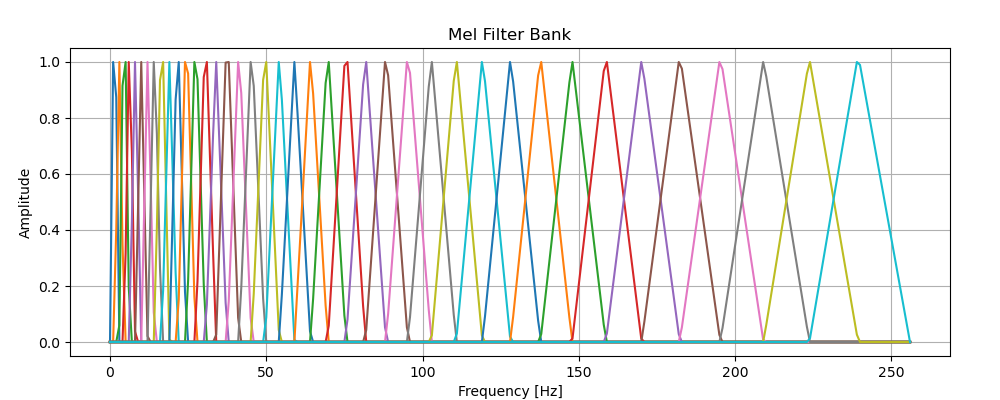
\includegraphics[width=0.5\textwidth]{D:/Project1/task1/Mel.png}
\caption{Mel滤波器}
\end{figure}

\subsubsection{MFCC特征}

MFCC(梅尔频率倒谱系数)也是一种广泛用于语音处理中的语音特征。其利用Mel刻度与信号频率的非线性对应关系,计算得到信号频率特征。MFCC可由FBank特征进一步计算得到,即在Fbank的基础上增加一个离散余弦变换(DCT)。计算公式如下:
\[MFCC(n) = \sum_{m=0}^{M-1}FBank(m)\cos\left[\frac{\pi}{M}n\left(m+\frac{1}{2}\right)\right]\]
其中$MFCC(n)$为第$n$个MFCC特征,$FBank(m)$为第$m$个FBank特征,$M$为FBank特征的维度。

\subsection{算法描述}

% 请描述你的语音端点检测算法。若不止一种,可继续分节。请尽可能使用伪代码描述。如有必要,可以
% 贴出少量程序代码。\textbf{写作完成后,请删除本段。}

\subsubsection{深度神经网络}

深度神经网络(DNN)是一种基于神经网络的分类器,通过多层神经元的连接,对输入数据进行特征提取和分类。在本次语音端点检测任务中,我们可以使用DNN分析MFCC特征与语音端点之间的关系。

\begin{algorithm}[H]
    \caption{深度神经网络}
    \begin{algorithmic}[1]
        \State\textbf{输入:}13维的MFCC特征
        \State\textbf{输出:}这一帧是语音信号的概率
        \State{输入层:13维MFCC特征}
        \State{隐藏层:64维全连接层}
        \State{输出层:1维,通过Sigmoid激活函数对输出归一化}
    \end{algorithmic}
\end{algorithm}

使用二分类交叉熵作为损失函数对网络进行训练。其计算公式如下:
\[Loss = -[y\cdot \log(\hat{y})+(1-y)\cdot \log(1-\hat{y})]\]
其中$Loss$为损失函数,$y$为真实标签,$\hat{y}$为预测标签。\\

使用Adam优化器对网络进行优化,其中学习率设置为$10^{-5}$,避免训练不收敛、正则化系数设置为$10^{-4}$,防止过拟合。

训练100轮,观察训练集和开发集上的损失函数变化,如下图所示:

\begin{figure}[H]
    \centering
  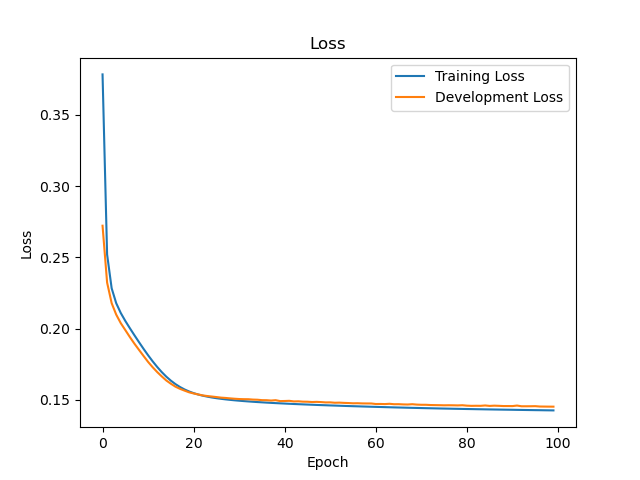
\includegraphics[width=0.4\textwidth]{D:/Project1/task2/损失曲线.png}
  \caption{损失函数变化}
\end{figure}

由损失函数变化曲线可看出,当训练到第100轮时,训练集和开发集上的损失函数均收敛且数值较低,说明模型已经训练完毕。

\subsubsection{优化预测结果}

与1.2.2.节类似,考虑到语音信号的连续性,可对预测结果进行优化,减少其中的断点。但由于DNN的输出是语音帧为语音信号的概率,故无法直接采用1.2.2.节的方法,而应用\verb|np.convolve()|函数对预测结果进行卷积平滑处理。

由参数调节得,使用\verb|np.ones(L)/L|作为卷积核,\verb|L|取23时,对预测结果的优化效果较好。

而由于DNN的输出是每个语音帧为语音信号的概率,我们可以通过设置一个阈值将其二值化,当概率大于阈值时,判断为语音信号。

由参数调节得,阈值取0.55时效果较好。

\begin{figure}[H]
    \centering
  \includegraphics[width=0.5\textwidth]{D:/Project1/task2/预测图.png}
  \caption{优化前后与真实标签对比图}
\end{figure}

\subsection{实验结果}

% 请使用表格等形式给出你的算法在开发集上的性能表现。\textbf{写作完成后,请删除本段。}

为验证该深度神经网络的性能,在开发集上进行测试,测试结果如下:

\begin{figure}[H]
    \centering
  \includegraphics[width=0.5\textwidth]{D:/Project1/task2/ROC.png}
  \caption{ROC曲线}
\end{figure}

\begin{table}[H]
    \caption{开发集测试结果}
    \centering
    \begin{tabular}{ l c r }
        \toprule
        \textbf{AUC} & \textbf{EER} & \textbf{ACC} \\
        \midrule
        0.9871 & 0.0557 & 0.9603 \\
        \bottomrule
    \end{tabular}
\end{table}

由测试结果可看出,该DNN在开发集上的性能表现比阈值分类器更好,ROC曲线下面积与准确率均更高,且等错误率更低。

\end{document}
